% Created 2023-01-20 Fri 14:34
% Intended LaTeX compiler: xelatex
\documentclass[11pt,twoside,landscape]{article}
\usepackage{graphicx}
\usepackage{longtable}
\usepackage{wrapfig}
\usepackage{rotating}
\usepackage[normalem]{ulem}
\usepackage{amsmath}
\usepackage{amssymb}
\usepackage{capt-of}
\usepackage{hyperref}
\usepackage{subcaption}
\usepackage[newfloat]{minted}
\usepackage{color}
\usepackage{listings}
\usepackage[top=2cm,bottom=2cm,right=2cm,left=2cm,landscape]{geometry}
\usepackage{multicol}
\usepackage{enumitem}
\usepackage{fancyhdr}
\usepackage{caption}
\usepackage{algorithm}
\usepackage{algpseudocode}
\usepackage{float}
\setlist{noitemsep}
\setlength{\parindent}{0pt}
\setlength{\columnseprule}{0.2pt}
\definecolor{mygreen}{rgb}{0,0.6,0}
\definecolor{mygray}{rgb}{0.5,0.5,0.5}
\definecolor{mymauve}{rgb}{0.58,0,0.82}
\lstset{ backgroundcolor=\color{white}, basicstyle=\footnotesize, breaklines=true, captionpos=b, commentstyle=\color{mygreen}, escapeinside={\%*}{*)},keywordstyle=\color{blue}, stringstyle=\color{mymauve},}
\author{Olivier Lischer}
\date{\today}
\title{AppArch Summary}
\hypersetup{
 pdfauthor={Olivier Lischer},
 pdftitle={AppArch Summary},
 pdfkeywords={},
 pdfsubject={},
 pdfcreator={Emacs 27.2 (Org mode 9.5.5)}, 
 pdflang={English}}
\begin{document}

\pagestyle{fancy}
\fancyhf{}
\fancyhead[R]{AppArch-HS22}
\fancyhead[L]{Summary}
\fancyfoot[CE,CO]{\leftmark}
\fancyfoot[R]{\thepage}
\fancyfoot[L]{Olivier Lischer}

\tableofcontents
\newpage

\begin{multicols}{3}
\section{Architecture Significance}
\label{sec:orgeeba1e8}
\subparagraph{Software Architecture} \
\label{sec:org13ea293}
Software Architecture is the organization of the system components with their relationships.
Design principles should help to make decisions how to create components and the relationships.


\begin{quote}
The fundamental organization of a system is embodied in its components,
their relationships to each other, and to the environment, and the
principles guiding its design and evolution.
-- [ISO/IEC/IEEE 42010, November 2011]
\end{quote}
\subparagraph{User Story} \
\label{sec:org6e48838}
User Stories describe a feature which should be implemented.
User Stories can often translate from \href{../../../roam/20230102105027-functional_requirements.org}{Functional Requirements}.


\begin{itemize}
\item As a (\textbf{who} wants to accomplish something)
\item I want to (\textbf{what} they want to accomplish)
\item So that (\textbf{why} they want to accomplish that thing)
\end{itemize}

An example:
\begin{itemize}
\item As a bank customer
\item I want to withdraw money from an ATM
\item So that I’m not constrained by opening hours or lines at the teller’s
\end{itemize}
\subparagraph{Architectural Significance of Requirements} \
\label{sec:org44690ac}
ASR are requirements (\href{../../../roam/20230102105027-functional_requirements.org}{Functional Requirements} or \href{../../../roam/20230102105647-non_functional_requirements.org}{Non-Functional Requirements}) which have a measurable impact on the systems' architecture.

\subparagraph{ASR Test} \
\label{sec:org5d5ad38}
With the ASR Test you can test / determine the architectural significance of requirements.
\textbf{Important}: They are not \href{../../../roam/20230102114435-mece.org}{MECE}.

\begin{enumerate}
\item The requirement is directly associated with high \textbf{business value} or \textbf{business risk}.
\item The requirement is a \textbf{concern} of a particularly important \textbf{stakeholder} (for instance, the project sponsor or an external compliance auditor).
\item The requirement has runtime \textbf{Quality-of-Service (QoS)} characteristics (e.g., performance needs) that deviate from those already satisfied by the evolving architecture substantially.
\item The requirement causes new or deals with one or more existing \textbf{external dependencies} that have unpredictable, unreliable and/or uncontrollable behavior.
\item The requirement has a \textbf{cross-cutting nature} and therefore affects multiple parts of the system and their interactions; it may even have system-wide impact.
\item The requirement has a \textbf{first-of-a-kind} character: e.g., the team has never built a component that satisfies this particular requirement.
\item The requirement has been \textbf{troublesome} and caused critical situations, budget overruns or client dissatisfaction \textbf{in a previous project} in a similar context.
\end{enumerate}

{
\begin{center}
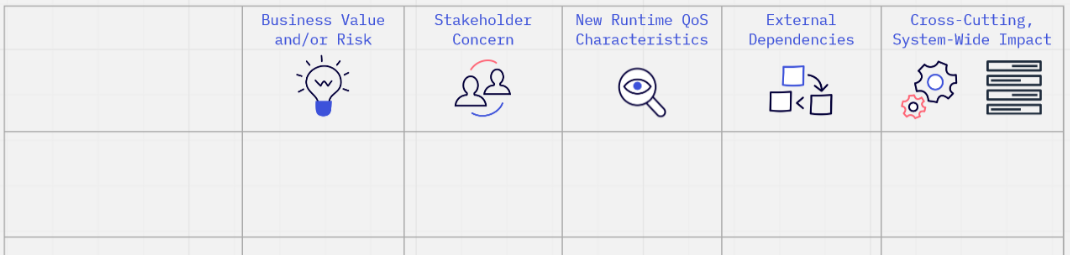
\includegraphics[width=.9\linewidth]{img/asr_template.png}
\end{center}
\captionof{figure}{Example for an ASR template}\label{fig:example-for-an-asr-template}
}
\subparagraph{SMART} \
\label{sec:org9ab77e8}
\textbf{SMART} are the letters


{
\begin{center}
\begin{tabular}{lll}
Letter & Project Mgmt & Requirements Engineering\\[0pt]
\hline
S & Specific & Specific\\[0pt]
M & Measurable & Measurable\\[0pt]
A & Achievable & Agreed Upon\\[0pt]
R & Relevant & Realistic\\[0pt]
T & Time-Bound & Time-Bound\\[0pt]
\end{tabular}
\end{center}
\captionof{table}{SMART Abbrevation Table}\label{tbl:smart-abbrevation-table}
}


\begin{description}
\item[{S}] Which feature of part of the system should satisfy the requirement?
\item[{M}] How can you find out whether the requirement is met (or not), is it quantified?
\end{description}
\section{Requirements}
\label{sec:org8cccf69}
\subparagraph{FURPS} \
\label{sec:org9bc0e3f}
\textbf{FURPS} is an acronym representing a model for classifying software quality attributes (\href{../../../roam/20230102105027-functional_requirements.org}{Functional Requirements} and \href{../../../roam/20230102105647-non_functional_requirements.org}{Non-Functional Requirements}).

FURPS:
\begin{description}
\item[{F}] Functionality
\item[{U}] Usability
\item[{R}] Reliability
\item[{P}] Performance
\item[{S}] Supportability
\end{description}


Plus (+)
\begin{itemize}
\item Design constraints
\item Implementation constraints
\item Physical constraints
\item Interface constraints
\end{itemize}
\subparagraph{Quality Attribute Scenario} \
\label{sec:orgfa49cae}
Quality Attribute Scenario (QAS) are \href{../../../roam/20230102105647-non_functional_requirements.org}{Non-Functional Requirements} which are very important (high impact).
For such requirements you could fill out the template as show in \autoref{fig:qas-template}.


\begin{itemize}
\item Stimulus:
\begin{itemize}
\item What starts the whole thing?
\end{itemize}
\item Stimulus Source:
\begin{itemize}
\item Who starts the whole thing?
\end{itemize}
\item Environment:
\begin{itemize}
\item In which situation (normal operation, stress operation, \ldots{})
\end{itemize}
\item Artifact:
\begin{itemize}
\item Everything what specified is
\end{itemize}
\item Response:
\begin{itemize}
\item An observable behavior
\end{itemize}
\item Response Measure
\begin{itemize}
\item Set measurable number as values
\end{itemize}
\end{itemize}


{
\begin{center}
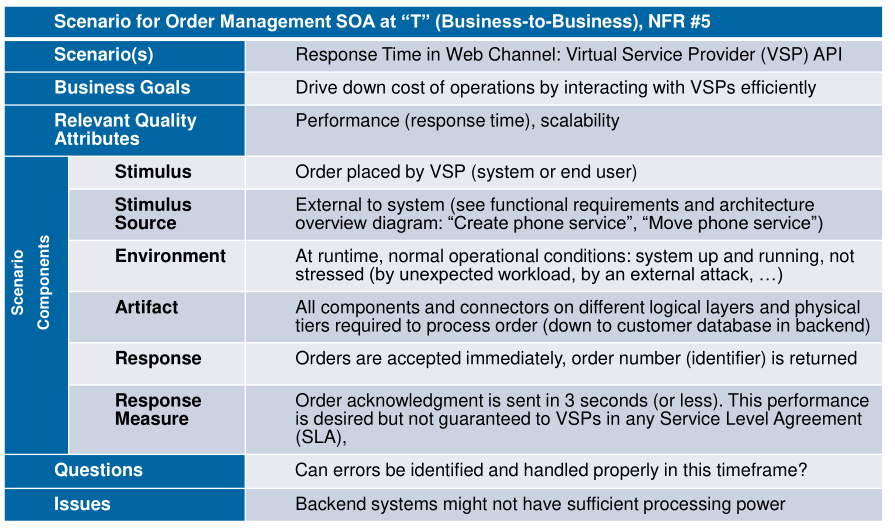
\includegraphics[width=.9\linewidth]{img/qas_template.png}
\end{center}
\captionof{figure}{QAS Template}\label{fig:qas-template}
}
\subparagraph{Agile Landing Zones} \
\label{sec:org8efead3}
Agile Landing Zones can be used to quantify \href{../../../roam/20230102105647-non_functional_requirements.org}{NFR}.
Instead of estimating a single value you estimate three values (M1, M2, M3).
Instead of aiming for a single value you have three values.

\begin{description}
\item[{M1}] Minimal Goal (you \textbf{HAVE} to meet this requirement)
\item[{M2}] Target (you plan for this goal)
\item[{M3}] Outstanding (you design for this goal)
\end{description}
\subparagraph{C4 Model} \
\label{sec:org29ee0d4}
The C4 Model consists of 4 different diagrams:
\begin{itemize}
\item Context
\item Container
\item Component
\item Classes
\end{itemize}


Each diagram zooms more and more into the class diagram.
\subparagraph{System Context Diagram} \
\label{sec:org07b6404}
A System Context Diagram (SCD) is used to define the boundary between systems, as part of the whole system and its relationship.
The Context Diagram from the C4 Model (\href{../../../roam/20230102124209-what_is_the_c4_model.org}{What is the C4 Model}) is such a SCD.
\section{Solution Strategy}
\label{sec:orgeedb822}
\subparagraph{Solution Strategy} \
\label{sec:orgef357f4}
\begin{quote}
Summary of the fundamental decisions and solution strategies that shape the architecture.
Can include technology, top-level decomposition, approaches to achieve top quality goals
and relevant organizational decisions.
\end{quote}


In Solution Strategy you will make big decisions as:
\begin{itemize}
\item client / server architecture
\item our application communicates over JSON
\begin{itemize}
\item JSON schema is not required to be defined at this stage
\end{itemize}
\end{itemize}


Solution Strategy will be performed during Inception \& Elaboration from \href{../../../roam/20220222103504-rational_unified_process.org}{RUP}.
\subparagraph{Architectural Decisions} \
\label{sec:org869c2bd}
Architectural Decisions are used to capture \textbf{key design} issues and the rationale behind chosen solutions.
These decisions can be documented with e.g. \href{../../../roam/20230102142920-what_are_y_statements.org}{Y Statements}
\subparagraph{Y Statements} \
\label{sec:org1cd2ac3}
The Y-Statement can be used to document \href{../../../roam/20230102130829-what_are_architectural_decisions.org}{Architectural Decisions}.
\textbf{Facing} and \textbf{to achieve} look very similar.
\textbf{Facing} talks about what is required / needed (by the client).
\textbf{To achieve} talks about what I want to solve with the solution.

\begin{quote}
\begin{itemize}
\item In the context of the order management scenario at T,
\item facing the need to process customer orders synchronously, without loosing any messages,
\item we decided to apply the Messaging pattern and the RPC pattern
\begin{itemize}
\item and neglected File Transfer, Shared Database, no physical distribution (local calls)
\end{itemize}
\item to achieve guaranteed delivery and request buffering when dealing with unreliable data sources
\item accepting that follow-on detailed design work has be performed and that we need to select, install, and configure a message-oriented middleware provider.
\end{itemize}
\end{quote}


{
\begin{center}
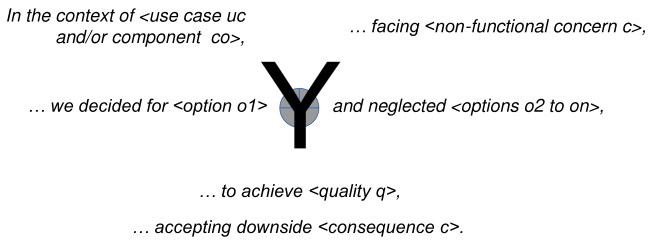
\includegraphics[width=.9\linewidth]{img/y_statements.png}
\end{center}
\captionof{figure}{Y-Statement Template}\label{fig:y-statement-template}
}
\section{Container Architecture}
\label{sec:org02bde22}
\subparagraph{Beans} \
\label{sec:org5bb7121}
Beans are self written components (see \href{../../../roam/20230102124209-what_is_the_c4_model.org}{C4 Model}).
\subparagraph{Inversion of Control (IoC)} \
\label{sec:org1579caa}
Inversion of Control is a design pattern which is often used by frameworks.
I write a component, and then I tell the framework how and when it should be called.

The Framework controls the workflow and calls your components when appropriate.
This is also called /Hollywood-Principle:
\begin{quote}
Don't call us, we call you!
\end{quote}

{
\begin{center}
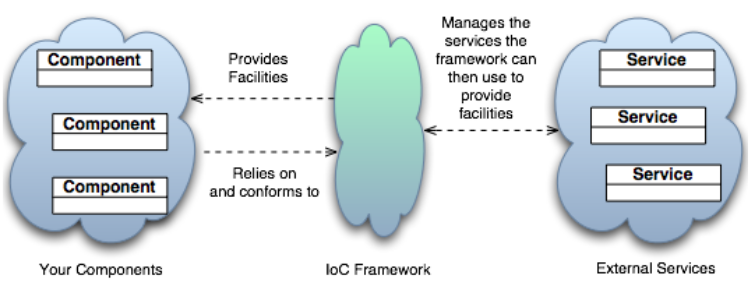
\includegraphics[width=.9\linewidth]{img/inversion_of_control.png}
\end{center}
\captionof{figure}{Example for IoC}\label{fig:example-for-ioc}
}
\section{Story Splitting}
\label{sec:orge4f60cc}
\subparagraph{INVEST} \
\label{sec:org1414752}
If a \href{../../../roam/20230102104722-what_is_a_user_story.org}{User Story} is too large for a sprint you have to brake it down.
The INVEST properties should help you:

\begin{description}
\item[{I}] Independent
\item[{N}] Negotiable
\item[{V}] Valuable
\item[{E}] Estimable
\item[{S}] Small
\item[{T}] Testable
\end{description}
\subparagraph{Story Splitting} \
\label{sec:org5f89cd0}
Sometimes a \href{../../../roam/20230102104722-what_is_a_user_story.org}{User Story} does not satisfy the \href{../../../roam/20230102161001-what_is_invest.org}{INVEST} criteria.
In these cases you should perform Story Splitting.
Story Splitting is the process of splitting a bad written User Story into many smaller and better User Stories. 

\subparagraph{Story Splitting: Example\hfill{}\textsc{ATTACH}} \
\label{sec:org6213288}
\begin{verbatim}
As a Virtual Service Provider (VSP) and client of “T”, I would like to create telephony orders
on behalf of my end customers rapidly and reliably to that they are satisfied and stay with
me rather than switch to T or another VSP.
\end{verbatim}

{
\begin{center}
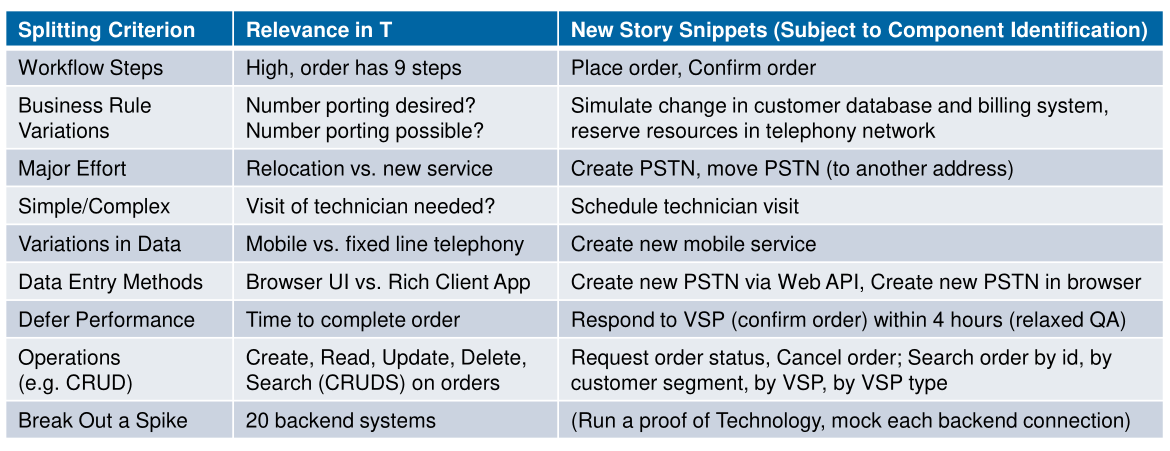
\includegraphics[width=.9\linewidth]{img/story_splitting_example.png}
\end{center}
\captionof{figure}{Example output after Story Splitting}\label{fig:example-output-after-story-splitting}
}
\section{Tactic DDD}
\label{sec:org689863f}
\subparagraph{Domain-Driven Design} \
\label{sec:org160b577}
Domain-Driven Design is a software design approach, focusing on modeling software to match a domain according to input from a domain's experts.

\begin{quote}
Under domain-driven design, the structure and language of software code (class names, class methods, class variables) should match the business domain.
For example, if software processes loan applications, it might have classes like loan application, customer, and methods such as accept offer and withdraw.
\end{quote}

Try to avoid naming like in \autoref{fig:aligning-organization-and-architecture-with-strategic-ddd}.

{
\begin{center}
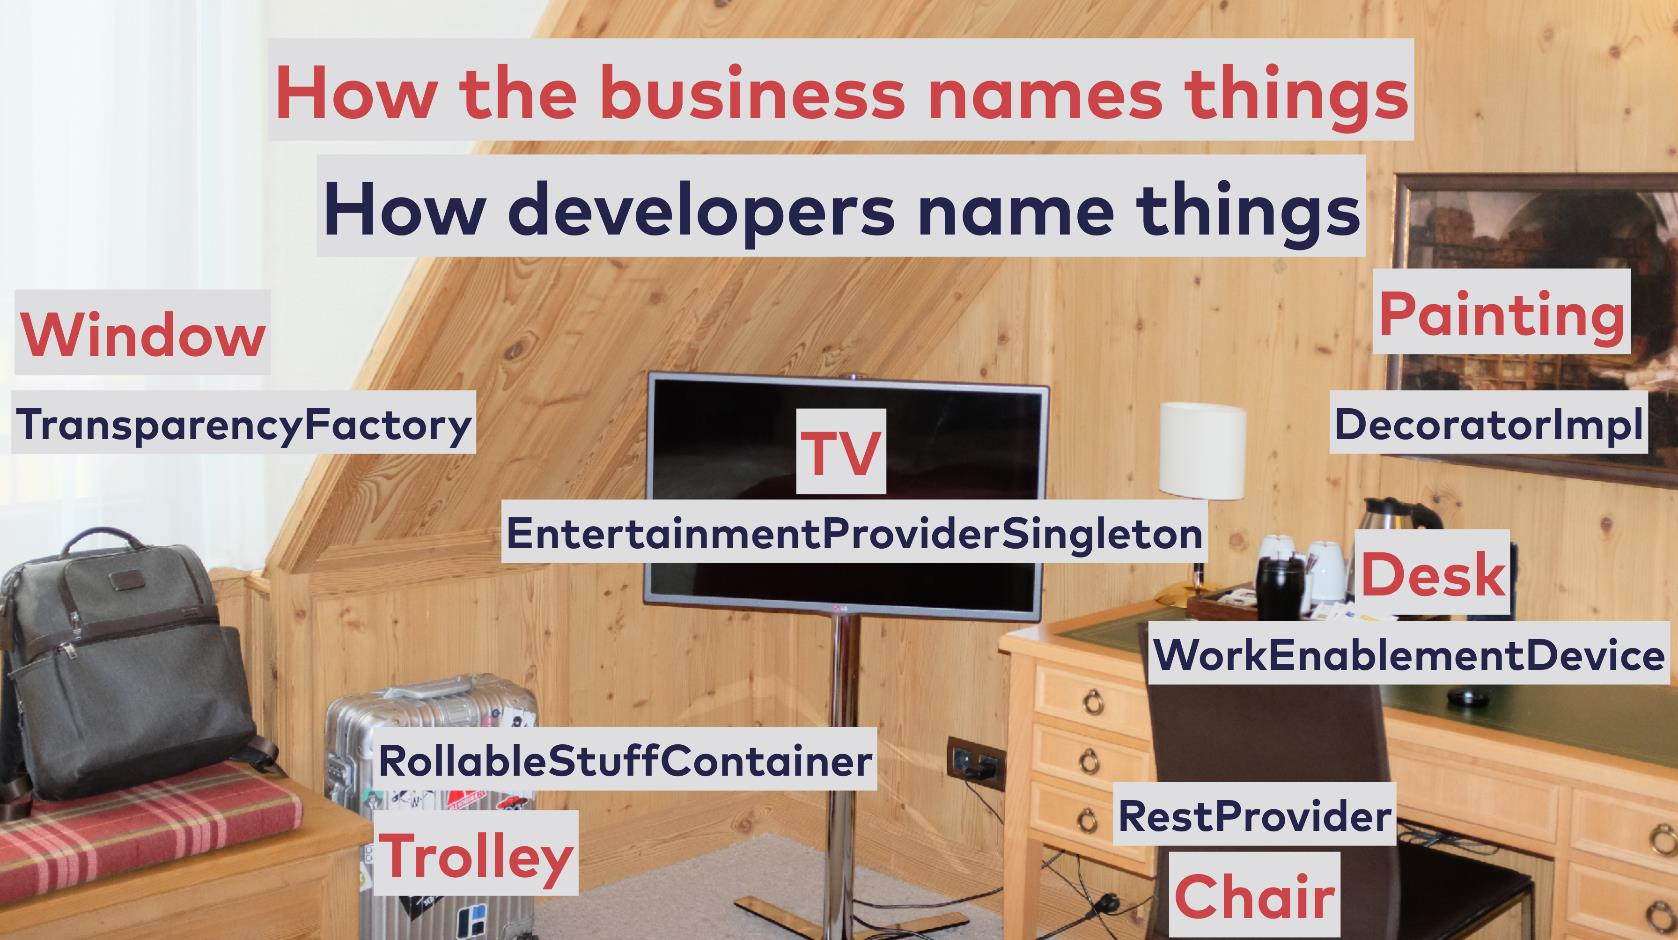
\includegraphics[width=.9\linewidth]{img/anti_ddd_naming.png}
\end{center}
\captionof{figure}{Aligning organization and architecture with strategic DDD}\label{fig:aligning-organization-and-architecture-with-strategic-ddd}
}
\subparagraph{Tactic DDD} \
\label{sec:orgf6571e9}
In tactic / tactical DDD you focus on how to build a \href{../../../roam/20211013171211-what_is_a_domain_model.org}{Domain Model} from a few basic building blocks.

\begin{description}
\item[{Entities}] A potentially changeable object with an identity (Person)
\item[{Value Objects}] An immutable object, without identity (int, char, \href{../../../roam/20230105183150-design_pattern_value_object.org}{Design Pattern - Value Object})
\item[{Aggregates}] Combines / Groups Entities \& Value Objects into cohesive units (Car consists of an Engine, Wheels, \ldots{})
\begin{itemize}
\item The parent \emph{Entity} of this cluster is called \emph{Aggregate Root}.
\end{itemize}
\item[{Services}] Stateless objects which performs logic not fitting in \emph{Entities} or \emph{Value Objects}
\item[{Repositories}] Are used to deal with storage. Used to save / load aggregates.
\item[{Factories}] Are used to build complex \emph{Entities}, \emph{Value Objects} or \emph{Aggregate Root}
\item[{Events}] An immutable representation of something that happened in the domain
\begin{itemize}
\item Often exchanged between \emph{Aggregates}
\end{itemize}
\end{description}


{
\begin{center}
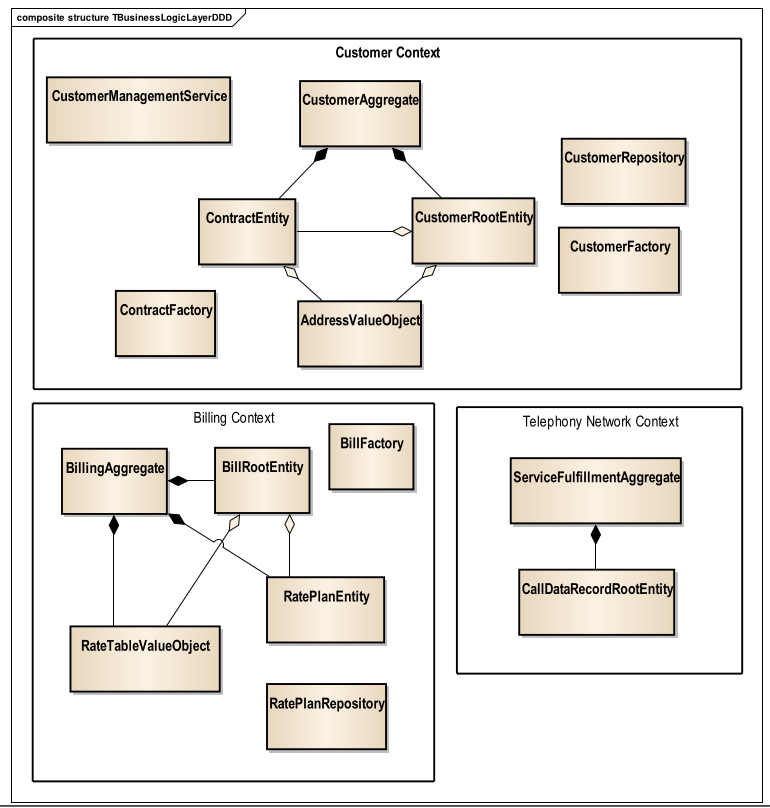
\includegraphics[width=.9\linewidth]{img/tactic_ddd_example.png}
\end{center}
\captionof{figure}{Tactic DDD Example}\label{fig:tactic-ddd-example}
}

{
\begin{center}
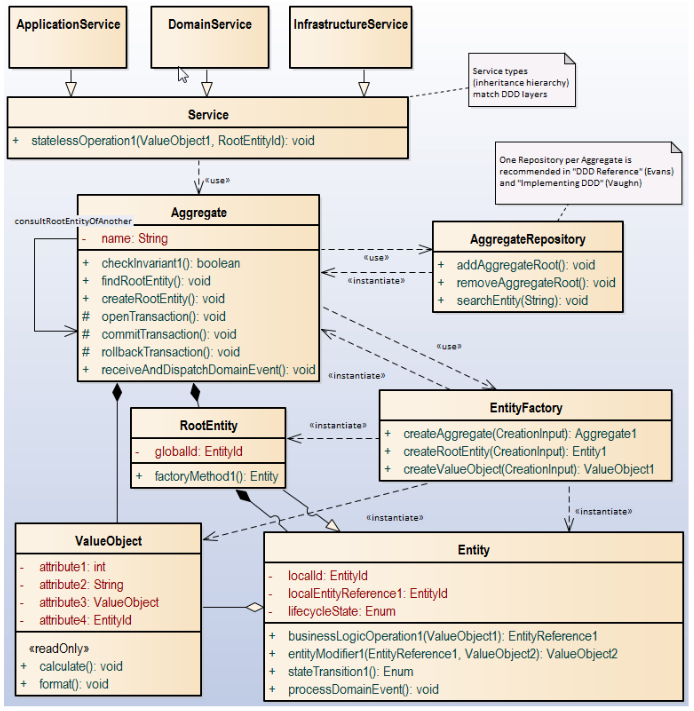
\includegraphics[width=.9\linewidth]{img/tactic_ddd_example_2.png}
\end{center}
\captionof{figure}{Tactic DDD Example 2}\label{fig:tactic-ddd-example-2}
}
\subparagraph{CRC Cards} \
\label{sec:org39396b9}
CRC Cards (Class-Responsibility-Collaboration Cards) is a brainstorming method to design and find components.
Original from the OO world, but is well suited for software architecture and web.

{
\begin{center}
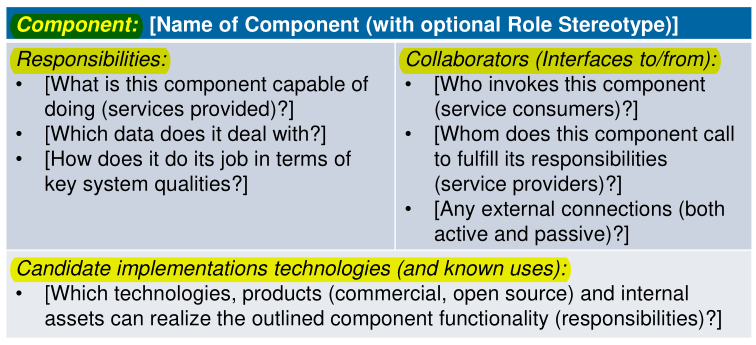
\includegraphics[width=.9\linewidth]{img/crc_template.png}
\end{center}
\captionof{figure}{CRC Card Template}\label{fig:crc-card-template}
}
\section{Strategic DDD}
\label{sec:orgbfdef5f}
\subparagraph{Business Rule} \
\label{sec:orgc5e52de}
A Business Rule has (at least) two meanings:
\begin{enumerate}
\item Executable part of the business logic (algorithm) which is expressed declarative
\begin{itemize}
\item if [cond.] then [do]
\item rules as in logical programming
\end{itemize}
\item A Statement or condition about the domain model
\begin{itemize}
\item E.g. the sum of all withdrawals is equal to the sum of all payments
\end{itemize}
\end{enumerate}
\subparagraph{Strategic DDD} \
\label{sec:org03b8324}
In Strategic DDD you will define
\begin{itemize}
\item Bounded Contexts
\item Ubiquitous Language
\item Context Map
\end{itemize}
\subparagraph{Bounded Context} \
\label{sec:org1cd2911}
When you try to model a big \href{../../../roam/20211013171211-what_is_a_domain_model.org}{Domain Model} you may encounter the problem that different groups use different terms.
A Bounded Context is mainly for linguistic purpose.
Each Bounded Context has its own \href{../../../roam/20230107180234-what_is_a_ubiquitous_language.org}{Ubiquitous Language}.

As your model evolves you may want to create relationships between Bounded Contexts.
For this we have the \href{../../../roam/20230107180425-what_is_a_context_map.org}{Context Map}.
\subparagraph{Ubiquitous Language} \
\label{sec:orgbe60f56}
Inside a \href{../../../roam/20230107175921-what_are_bounded_context.org}{Bounded Context} you speak a ubiquitous language.
This language is determined in collaboration with the whole team and the domain expert.
The language should uniquely identify each concept in this context (sub domain).
\subparagraph{Context Map} \
\label{sec:org12bd981}
In a big \href{../../../roam/20211013171211-what_is_a_domain_model.org}{Domain Model} you will have multiple \href{../../../roam/20230107175921-what_are_bounded_context.org}{Bounded Context}.
At some point you have to bring this Bounded Context in a relationship.
The context map should help here.


The Context Map has the following relationships:
\begin{description}
\item[{Shared Kernel (SK)}] Two bounded contexts use a common kernel of code (for example a library)
\item[{Open Host Service (OHS)}] A Bounded Context specifies a protocol by which any other bounded context can use its services (e.g. RESTful HTTP)
\item[{Published Language (PL)}] The interacting bounded contexts agree on a common a language (for example a bunch of XML or JSON schemas)
\item[{Conformist (CF)}] BC uses the services of another but is not a stakeholder (e.g. public API)
\item[{Anti-Corruption Layer (ACL)}] BC uses the services of another but is not a stakeholder (e.g. public API).
But has build a layer to minimize impact from changes in the other bounded context.
\item[{Customer/Supplier (CS)}] BC uses the services of another but is a stakeholder (customer).
It can influence the development in the other BC.
\end{description}


The relation also needs to specify how the data flow is:
\begin{quote}
an upstream context will influence the downstream counterpart while the opposite might not be true.
This might apply to code (libraries depending on one another) but also on less technical factors such as schedule or responsiveness to external requests.
\end{quote}


{
\begin{center}
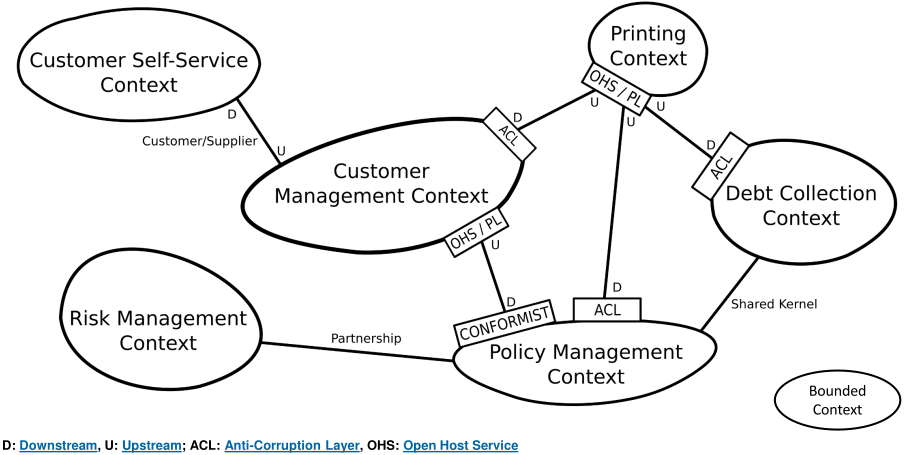
\includegraphics[width=.9\linewidth]{img/context_map_example.png}
\end{center}
\captionof{figure}{Context Map Example}\label{fig:context-map-example}
}
\section{Messaging}
\label{sec:org769a3f8}
\subparagraph{Lose Coupling} \
\label{sec:orga29c116}
Loose coupling means that two or more components does not depend on each strictly.
Every component could be replaced if desired.

Loose coupling has (at least) four dimensions:
\begin{itemize}
\item Reference autonomy (aka. location transparency)
\begin{itemize}
\item producer \& consumer don't know each other
\end{itemize}
\item Platform autonomy
\begin{itemize}
\item Producer \& consumer may be located in different technical environments, different languages
\end{itemize}
\item Time autonomy
\begin{itemize}
\item producer \& consumer access channel at their own pace
\end{itemize}
\item Format autonomy
\begin{itemize}
\item Producers \& consumer may use different formats of data exchanged
\end{itemize}
\end{itemize}

\subparagraph{Integration Styles} \
\label{sec:org827e735}
Integration Styles are used to communicate between different components.
A few examples:
\begin{description}
\item[{File Transfer}] e.g. \texttt{java.io} or FTP
\item[{Shared Database}] e.g. JDBC/SQL
\item[{Remote Procedure Call/Invocation (RPC, CPI)}] e.g. Java RMI, \href{../../../roam/20220704074452-grpc.org}{gRPC}
\item[{Messaging}] e.g. JMS, RabbitMQ
\end{description}
\subparagraph{Integration Style Messaging} \
\label{sec:org517078d}
A message is transmitted in five steps:
\begin{enumerate}
\item Create: the sender creates the message
\item Send: the sender adds the message to a channel
\item Deliver: the messaging system moves the message from sender to receiver
\item Receive: the receiver reads the message from the channel
\item Process: the receiver extracts the data from the message
\end{enumerate}


The Messaging Pattern has many variations.

{
\begin{center}
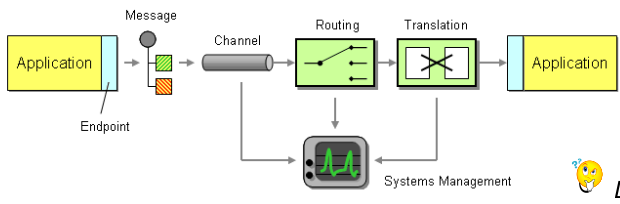
\includegraphics[width=.9\linewidth]{img/enterprise_integration_messaging.png}
\end{center}
\captionof{figure}{Enterprise Integration/Messaging}\label{fig:enterprise-integration-messaging}
}

\begin{description}
\item[{Document Message Pattern}] Send Document (JSON, XML)
\item[{Command Message Pattern}] Command Message to invoke a procedure in another application
\item[{Point-to-Point Channel}] Only one receiver will receive a particular message
\item[{Publish-Subscribe Channel}] A sender sends the message to many receivers
\end{description}
\subparagraph{AMQP} \
\label{sec:orgb07c7e2}
AMQP is a Peer-to-Peer Transport Protocol operating over TCP for message-oriented middleware.
AMQP is a great protocol to use the \href{../../../roam/20230108144047-what_is_the_integration_style_messaging.org}{Messaging} Integration Style.
\section{Microservices}
\label{sec:org973ffad}
\subparagraph{Service vs Components} \
\label{sec:orgaea57cd}
A Component is a piece of software which can be used by foreign applications without changing its source code (e.g. JAR, DLL, \ldots{}).
A Service is similar to a component, but you will use it remotely through some remote interface (\href{../../../roam/20220704074452-grpc.org}{gRPC}, \href{../../../roam/20230108144047-what_is_the_integration_style_messaging.org}{Messaging}, \ldots{}).
\subparagraph{Clean Architecture} \
\label{sec:org021609c}
In the clean architecture you have rings.
The further out the code is, the more volatile it is.
The more in the center, the more stable is the code.
So your domain code is in the center and at the outer ring are things like UI frameworks.

{
\begin{center}
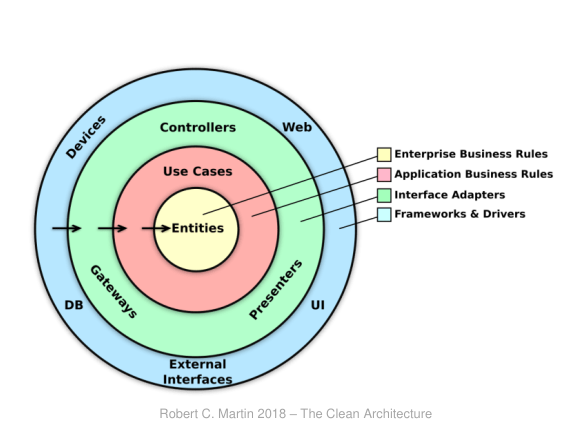
\includegraphics[width=.9\linewidth]{img/the_clean_architecture.png}
\end{center}
\captionof{figure}{Clean Architecture}\label{fig:clean-architecture}
}
\subparagraph{Hexagonal Architecture} \
\label{sec:org45722fc}
The Hexagonal Architecture / Onion Architecture / Ports and Adapters Pattern is a way how you can structure your application.

On the outside are the \emph{adapters}.
Adapters are concrete and are using libraries, services, databases, \ldots{}
In the inside are the \emph{ports}.
They are not interested in the concrete service / component (\href{../../../roam/20230108155804-what_are_the_differences_between_components_and_services.org}{What are the differences between components and services}).
Therefor, you implement against interfaces (\href{../../../roam/20220102152742-dependency_inversion_principle.org}{dependency inversion principle}).


{
\begin{center}
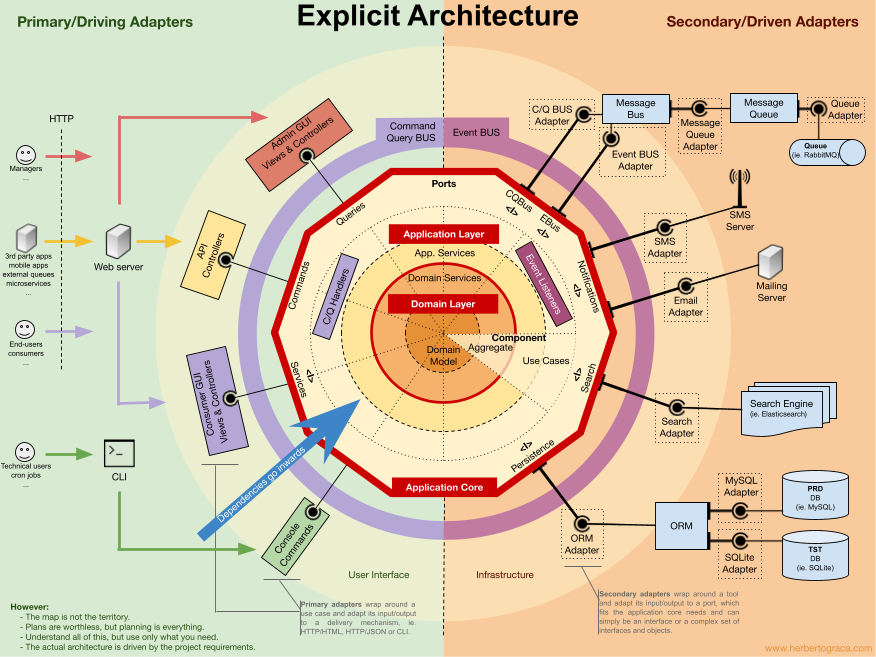
\includegraphics[width=.9\linewidth]{img/hexogonal_explicit_architecture.png}
\end{center}
\captionof{figure}{Hexagonal Architecture}\label{fig:hexagonal-architecture}
}
\subparagraph{Service-Oriented Architecture} \
\label{sec:orgce29422}
Service-Oriented Architecture is:
\begin{itemize}
\item a set of services and operations (Business Domain Analyst)
\item an architectural style (IT Architect)
\item a set of architectural patterns (IT Architect)
\item a programming and deployment model (Developer, Administrator)
\end{itemize}
\subparagraph{Microservices} \
\label{sec:org8a8bb43}
Microservices is an architecture type consists of many
\begin{itemize}
\item independently deployable
\item scalable
\item changeable
\end{itemize}
services.

Each service encapsulates and manages its \emph{own} store and communicates via message-based remote APIs (\href{../../../roam/20230108144047-what_is_the_integration_style_messaging.org}{Messaging}).
Idealy in a loosely coupled fashion (\href{../../../roam/20230108141515-what_does_loose_coupling_mean.org}{What does loose coupling mean}).
\subparagraph{Pro / Con Microservices} \
\label{sec:org0aa3925}
Pros:
\begin{itemize}
\item single components can be scaled
\item support for agile software development and continues delivery
\item well suited for implementing ‘IDEAL’ cloud-native applications
\item allows an incremental migration of monolithic applications
\end{itemize}


Cons:
\begin{itemize}
\item communication overhead within a distributed architecture
\item requires a disciplined approach to their life cycle management, monitoring, and debugging
\item single points of failure and cascading failure proliferation effects need to be avoided
\item data consistency and state management challenges are introduced
\item autonomy and consistency for the whole microservice architecture cannot be both guaranteed
\end{itemize}
\subparagraph{REST} \
\label{sec:org7f811aa}
REST is an architectural style (for integration), defined via constraint.
To be a REST conform you have to follow the following constraints:
\begin{itemize}
\item client-server
\item stateless
\item cacheable
\item uniform interface (URI, HTTP)
\item layered system
\item code on demand (optional)
\end{itemize}


To be RESTFul you have also to satisfy the next four constraints:
\begin{itemize}
\item identification of resources
\item manipulation of resources through representations
\item self-descriptive messages
\item hypermedia as the engine of application state (HATEOAS)
\end{itemize}
\subparagraph{REST Maturity Levels} \
\label{sec:org385d0b4}
An API on the web can be on different maturity levels:

\begin{itemize}
\item Level 0: The Swamp of POX (Plain Old XML Objects)
\begin{itemize}
\item Send data in an arbitrary way with XML / JSON objects
\end{itemize}
\item Level 1: Resources / HTTP Resource API (by Olaf Zimmermann)
\begin{itemize}
\item You have meaningful URLs
\end{itemize}
\item Level 2: HTTP Verbs / Web API (by Olaf Zimmermann)
\begin{itemize}
\item You use the HTTP Verbs (GET, POST, \ldots{}) in the correct way
\end{itemize}
\item Level 3: RESTFul HTTP / Hypermedia API (by Olaf Zimmermann)
\begin{itemize}
\item Navigation using links in response
\item They must contain application (flow) state
\end{itemize}
\end{itemize}


{
\begin{center}
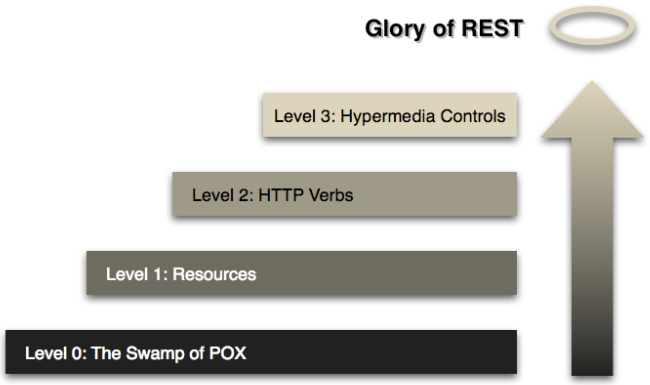
\includegraphics[width=.9\linewidth]{img/rest_maturity_levels.png}
\end{center}
\captionof{figure}{REST Maturity Levels}\label{fig:rest-maturity-levels}
}
\subparagraph{HATEOAS} \
\label{sec:org1509a50}
HATEOAS (Hypermedia As The Engine Of Application State) is constraint of the \href{../../../roam/20230108172748-what_is_rest.org}{RESTFul} style.
In HATEOAS the server provides the possible next actions in the request in form of links (see \autoref{lst:http-response})

\begin{lstlisting}[language=restclient,label=lst:http-response,caption={HTTP Response},captionpos=b,numbers=none]
HTTP/1.1 200 OK
Content-Type: application/vnd.acme.account+json
Content-Length: ...

{
    "account": {
	"account_number": 12345,
	"balance": {
	    "currency": "usd",
	    "value": 100.00
	},
	"links": {
	    "deposit": "/accounts/12345/deposit",
	    "withdraw": "/accounts/12345/withdraw",
	    "transfer": "/accounts/12345/transfer",
	    "close": "/accounts/12345/close"
	}
    }
}
\end{lstlisting}
\subparagraph{From Monolith and Components to SOA} \
\label{sec:org0556d98}
\begin{itemize}
\item \textbf{Monolitich application} aka the big ball of mud
\item \textbf{Internally componentized application}
\begin{itemize}
\item \emph{Logic} könnte ein Aggregate sein!
\item modular monolith
\end{itemize}
\item \textbf{Microservices application}
\end{itemize}

\section{API Description}
\label{sec:org2a96e09}
\subparagraph{Describe API} \
\label{sec:org2e9bf9b}
To describe / document an API at least 3 information are required:
\begin{itemize}
\item API Endpoint Information (e.g. URL / URI / \ldots{})
\item Operation Names (e.g. HTTP verbs)
\item Message Content (structure and meaning, e.g. using MIME, Content Type)
\end{itemize}


A more complete description / documentation contains a few additional information:
\begin{itemize}
\item Parameter Data Types (string, int, object, \ldots{})
\item Usage Examples
\item Error Codes and Reports
\item Compliance Test Cases
\item Behavior
\item Versioning Metadata
\end{itemize}
\subparagraph{Interface Definition Language} \
\label{sec:orgd2fda33}
An Interface Definition Language is used to describe an API in a \href{../../../roam/20210920103254-programming_language.org}{Programming Language} independent way.
One of the most common one for \href{../../../roam/20230108172748-what_is_rest.org}{REST} APIs is \href{../../../roam/20230111084434-openapi_specification.org}{OpenAPI Specification}.
An alternative WDSL (Web Services Description Language).
\subparagraph{OpenAPI Specification} \
\label{sec:orgfdc6127}
The OpenAPI Specification (OAS) is an \href{../../../roam/20230111084138-what_is_an_interface_definition_language.org}{IDL} to describe \href{../../../roam/20230108172748-what_is_rest.org}{REST} APIs.
The OpenAPI Specification is often written in JSON or YAML.
\section{Service Granularity}
\label{sec:org2352d49}
\subparagraph{Service Granularity} \
\label{sec:orgcfa8dbc}
Service Granularity is the size of a service.

\begin{quote}
Granularity is not defined by the number of classes or lines of code in a
service, but rather what the service does. -- Dr. Gerald Reif
\end{quote}

To find the right size / granularity for a service we have \href{../../../roam/20230111100624-what_are_service_granularity_integrators.org}{Service Granularity Integrators} and \href{../../../roam/20230111100600-what_are_service_granularity_disintegrators.org}{Service Granularity Disintegrators}.
\subparagraph{Service Granularity Disintegrators} \
\label{sec:orga542bca}
Provide guidance and justification for when to break a service into smaller pieces.

\begin{description}
\item[{Service scope and function}] Is the service doing too many unrelated things?
\item[{Code volatility}] Are changes isolated to only one part of the service?
\item[{Scalability and throughput}] Do parts of the service need to scale differently?
\item[{Fault tolerance}] Are there errors that cause critical functions to fail within the service?
\item[{Security}] Do some parts of the service need higher security levels than others?
\item[{Extensibility}] Is the service always expanding to add new contexts?
\end{description}
\subparagraph{Service Granularity Integrators} \
\label{sec:orgdcd15ba}
Provide guidance and justification for putting services back together (or not breaking apart a service in the first place).


\begin{description}
\item[{Database transactions}] Is an \href{../../../roam/20221121133858-acid.org}{ACID} transaction required between separate services?
\item[{Workflow and choreography}] Do services need to talk to one another?
\item[{Shared code}] Do services need to share code among one another?
\item[{Database relationships}] Although a service can be broken apart, can the data it uses be broken apart as well?
\end{description}
\subparagraph{Async vs sync} \
\label{sec:org2dc4079}
Two services can communicate in a synchronous or asynchronous (\href{../../../roam/20211207194612-async_vs_parallel.org}{async vs parallel}) manner.
Both have their pros and cons.

sync contra:
\begin{itemize}
\item performance impact on highly interactive systems
\item creates dynamic entanglements
\item creates limitations in distributed architectures
\end{itemize}


sync pro:
\begin{itemize}
\item easy to model transactional behavior
\item mimics non-distributed method calls
\item easier to implement
\end{itemize}


async contra:
\begin{itemize}
\item complex to build and debug
\item presents difficulties for transactional behaviors
\item error handling
\end{itemize}


async pro:
\begin{itemize}
\item allows highly decoupled systems
\item common performance tuning technique
\item high performance and scale
\end{itemize}
\subparagraph{Orchestrator} \
\label{sec:org5bd0178}
An Orchestrator implements the whole workflow logic.
The different services are not communicating directly, but over the orchestrator.
This is an implementation of the \href{../../../roam/20220413201546-design_pattern_mediator.org}{Design Pattern - Mediator}.

{
\begin{center}
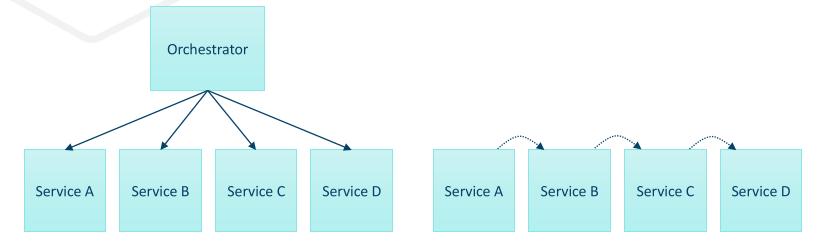
\includegraphics[width=.9\linewidth]{img/orchestrator_vs_choreography.png}
\end{center}
\captionof{figure}{orchestration vs choregraphy}\label{fig:orchestration-vs-choregraphy}
}
\subparagraph{orchestration vs choreography} \
\label{sec:org48acb15}
orchestration contra:
\begin{itemize}
\item slow responsiveness
\item fault tolerance (\href{../../../roam/20230111110301-what_is_an_orchestrator.org}{Orchestrator} down, everything down)
\item scalability (Orchestrator not easy scalable)
\item service coupling (Orchestrator has to know every service)
\end{itemize}


orchestration pro:
\begin{itemize}
\item centralized workflow
\item error handling (single point for error handling)
\item recoverability (knows everything, greater change to recover)
\item state management (management in a single point)
\end{itemize}


choreography contra:
\begin{itemize}
\item distributed workflow (Workflow is distributed over all services)
\item state management (difficult because no single place for state)
\item error handling (every service has to it by itself)
\item recoverability (difficult because service knows only its own information)
\end{itemize}


choreography pro:
\begin{itemize}
\item responsiveness (first service can react immediately)
\item fault tolerance (single service down, other services works)
\item scalability (you can scale each service individually)
\item service coupling (each service only has to know the service which communicates with)
\end{itemize}
\subparagraph{atomicity vs eventual consistency} \
\label{sec:org15f6be5}
\emph{Atomicity} guaranties that each transaction is treated as a single "unit".
This unit succeeds completely or fails completely.

\emph{Eventual Consistency} guaranties if no new updates are made to a given data item, eventually all access to that item will return the last updated value.
Language: [en] eventual -> [de] schlussendlich, irgendwann, letzten Endes – \textbf{Nicht eventuell!}
\section{Session State}
\label{sec:org02ea72e}
\subparagraph{Session State Management} \
\label{sec:org0bc6c7a}
In general there exists 3 types how / where you can manage / store state:
\begin{itemize}
\item Client Session State (REST Level 3)
\begin{itemize}
\item cookies, hidden fields, URL (for REST no cookies!), JWT
\end{itemize}
\item Server Session State
\begin{itemize}
\item uses main memory of the application server
\item not recommended because you very difficult to scale
\end{itemize}
\item Database Session State
\begin{itemize}
\item database and service can be scaled separately
\end{itemize}
\end{itemize}
\section{Patterns}
\label{sec:org900d0fe}
\subparagraph{Architecture Pattern - Layering} \
\label{sec:org5bedbac}
\begin{description}
\item[{Context}] A system that needs to be segmented due to its size and specialization.
\item[{Problem}] System design that supports a mixture of tasks on different levels.
\item[{Solution}] Organize the system into cohesive layers that are stacked on top of each other.
\end{description}


This pattern is often applied twice (logical and physical).
Logical layers (layers):
\begin{itemize}
\item presentation layer
\item business logical layer
\item data access layer
\end{itemize}

Physical layers (tiers)
\begin{itemize}
\item Browser
\item Application Server
\item Database Server
\end{itemize}
\subparagraph{Architecture Pattern - Distribution Pattern} \
\label{sec:org96f7ff4}
The Distribution Pattern describes how you can partition your application in client and server components.

\begin{itemize}
\item \href{../../../roam/20230107150231-distribution_pattern_remote_user_interface.org}{Distribution Pattern - Remote User Interface}
\item \href{../../../roam/20230107150503-distribution_pattern_distributed_presentation_layer.org}{Distribution Pattern - Distributed Presentation Layer}
\item \href{../../../roam/20230107150808-distribution_pattern_distributed_application_kernel.org}{Distribution Pattern - Distributed Application Kernel}
\item \href{../../../roam/20230107151100-distribution_pattern_remote_database.org}{Distribution Pattern - Remote Database}
\item \href{../../../roam/20230107151436-distribution_pattern_distributed_database.org}{Distribution Pattern - Distributed Database}
\end{itemize}
\subparagraph{Distribution Pattern - Remote User Interface} \
\label{sec:org25900a3}
In \emph{Remote User Interface} the tier 1 runs dialog control sub-layer (the C and the M in MVC) in addition to display.
An example for this pattern are today's Single-Page Applications (\href{../../../roam/20220513105545-javascript.org}{JavaScript} performs calls to API).
\subparagraph{Distribution Pattern - Distributed Presentation Layer} \
\label{sec:org41cb372}
In the \emph{Distributed Presentation Layer} the tier 1 client only renders display elements (the V in MVC).
Tier 2 owns/controls screen/page flow.

Example for this pattern are traditional (MVC) PHP application.
\subparagraph{Distribution Pattern - Distributed Application Kernel} \
\label{sec:org2656a87}
In the \emph{Distributed Application Kernel} pattern the business logic is \textbf{physically} distributed.
An example for this pattern are \href{../../../roam/20230107150950-what_are_microservices.org}{Microservice}.
\subparagraph{Distribution Pattern - Remote Database} \
\label{sec:org2ba1310}
In the \emph{Remote Database} pattern you use a Remote Database Access Protocol to connection your application to the database.
Example for this is JDBC/ODBC (Java) or sqlx (Rust, Go).
The transaction management is performed by the database itself.
\subparagraph{Distribution Pattern - Distributed Database} \
\label{sec:org3b5c399}
In the \emph{Distribution Database} your database is partitioned and/or partially replicated.
This can be done using a \href{../../../roam/20230107151606-what_is_a_two_phase_commit.org}{Two-Phase Commit} with an external transaction manager.
\subparagraph{Design Pattern - Template View} \
\label{sec:org32bd2f1}
You insert markers in the markup (for example HTML).
These markers are then replaced at runtime with real values.
Known uses are:
\begin{itemize}
\item Handelbars (JS)
\item tera (Rust)
\end{itemize}

\begin{quote}
Renders information into HTML by embedding markers in an HTML page.
\end{quote}
\section{END}
\label{sec:org08e3363}
\end{multicols}
\end{document}